\documentclass[a4paper]{article}
\usepackage[utf8]{inputenc}
\usepackage{fullpage}
\usepackage{enumitem}
\usepackage{todonotes}
\usepackage{graphicx}
\usepackage{array}
\usepackage{mdwlist}
\usepackage{floatrow}
\usepackage{hyperref}
\usepackage{listings}
\usepackage{color}

\graphicspath{ {img/} }

% New page before new section
\let\stdsection\section
\renewcommand\section{\newpage\stdsection}

% Set caption position
\floatsetup[figure]{capposition=bottom}

\title{{\Huge myTaxiService} \\ Design Document}
\author{Jacopo Strada \and Luca Riva}
\date{December 4, 2015}

\begin{document}

\maketitle

\newpage

\tableofcontents

\listoffigures 

\listoftables

\setlength{\parindent}{0em}
\setlength{\parskip}{1em}

\section{Introduction}
This system design document describes the main design concerns and will have an important role in the development and in the future maintenance of the software itself. The document is addressed to the city government and in particular to its IT department, since many diagrams, architectures and patterns references will be found in the next sections.

\subsection{Purpose}
The purpose of this document is to explain as clearly as possible every factor that may have created some perplexity in the client.

\subsection{Scope}
In the document it is discussed the interaction between the system and the actors, at the same time it is possible to find a detailed description of the communication among various components of the system executing certain operations.
\subsection{Glossary}
\subsubsection{Definitions}
\subsubsection{Acronyms}
\subsubsection{Abbreviations}
\subsection{Reference Documents}

\subsection{Document Structure}

\section{Architectural Design}
\subsection{Overview}
\subsection{High level components and their interaction}

\subsection{Component view}

\begin{figure}[H]
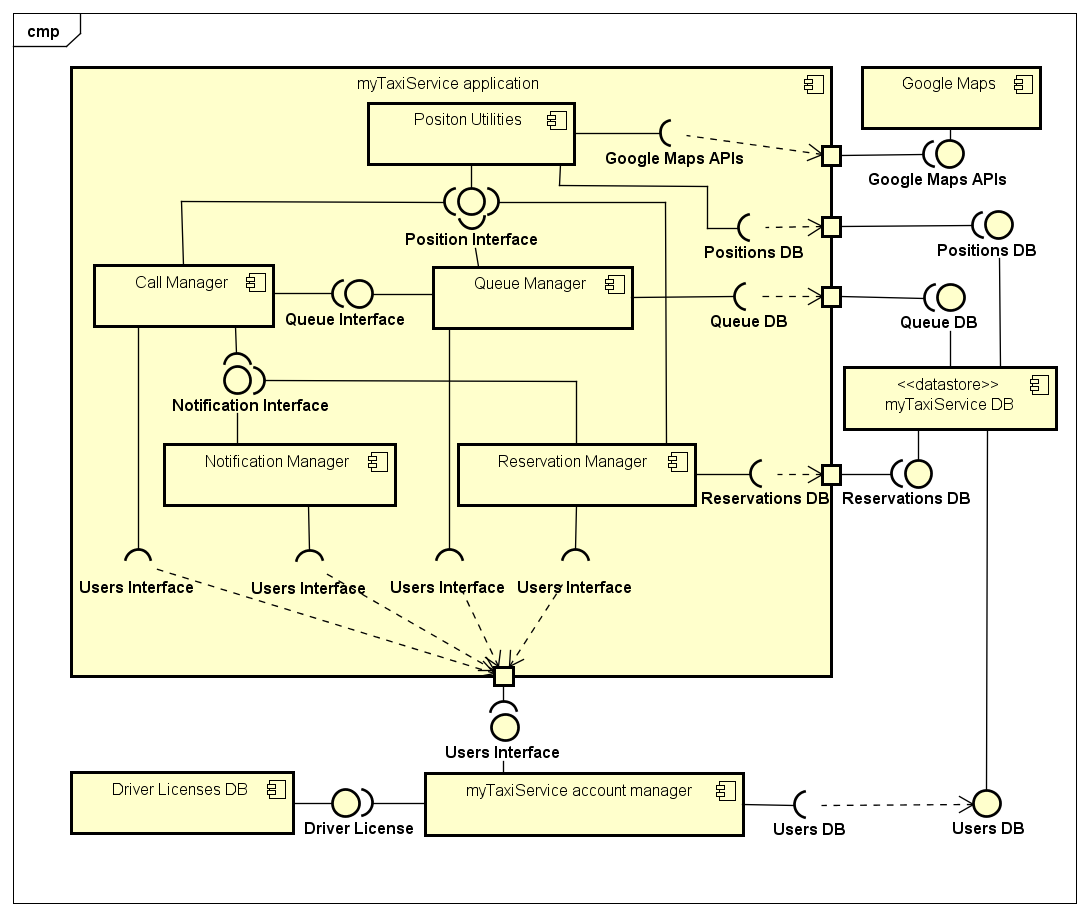
\includegraphics[width=.9\textwidth]{ComponentDiagram}
\centering
\caption{UML Component Diagram}
\label{fig:componentsiagram}
\end{figure}

\subsection{Deployment view}

\begin{figure}[H]
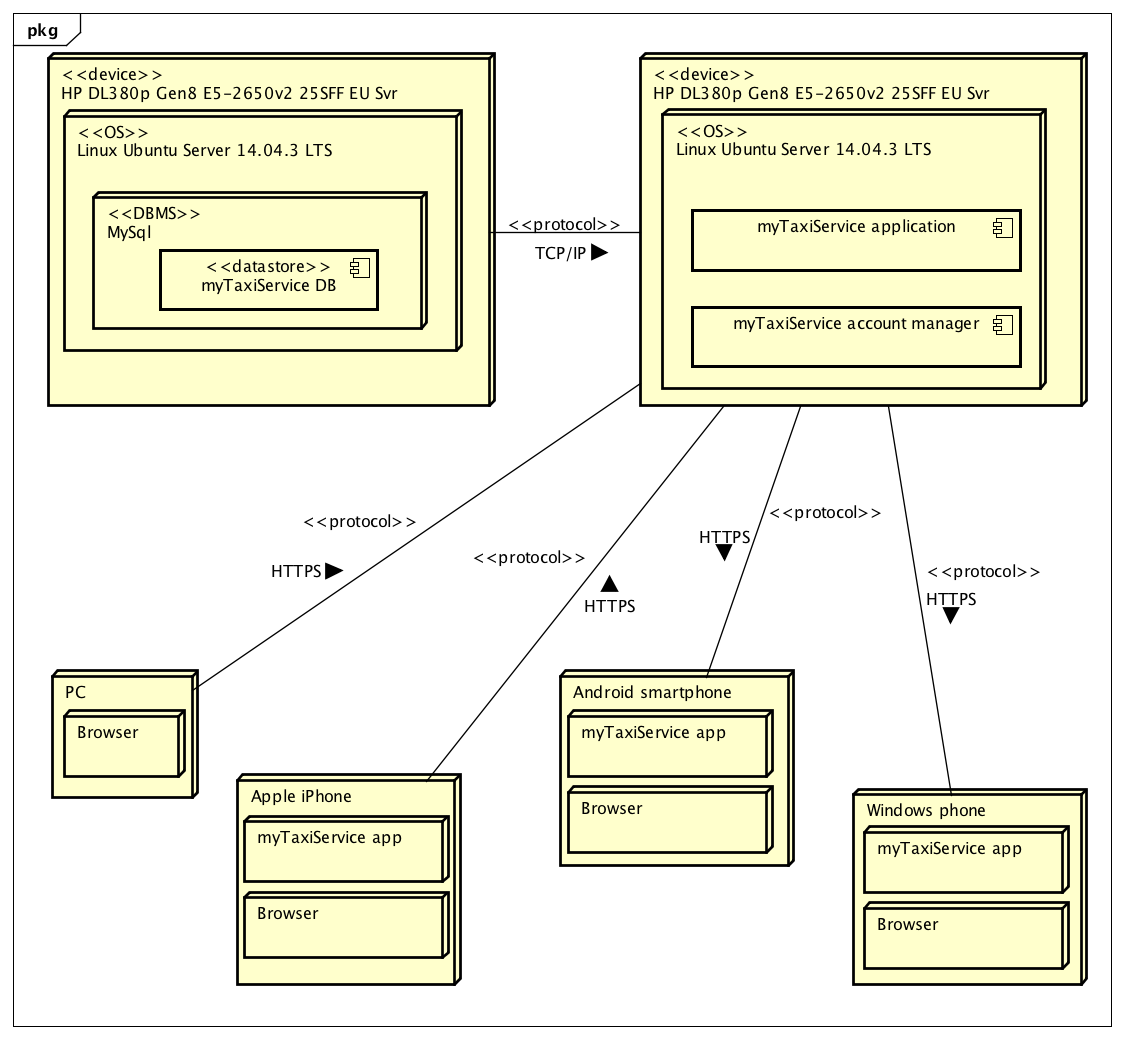
\includegraphics[width=.9\textwidth]{DeploymentDiagram}
\centering
\caption{UML Deployment Diagram}
\label{fig:deploymentsiagram}
\end{figure}

\subsection{Runtime view}

% Sequences Width
\newlength{\sequenceWidth}
\setlength{\sequenceWidth}{\textwidth}

\begin{figure}[H]
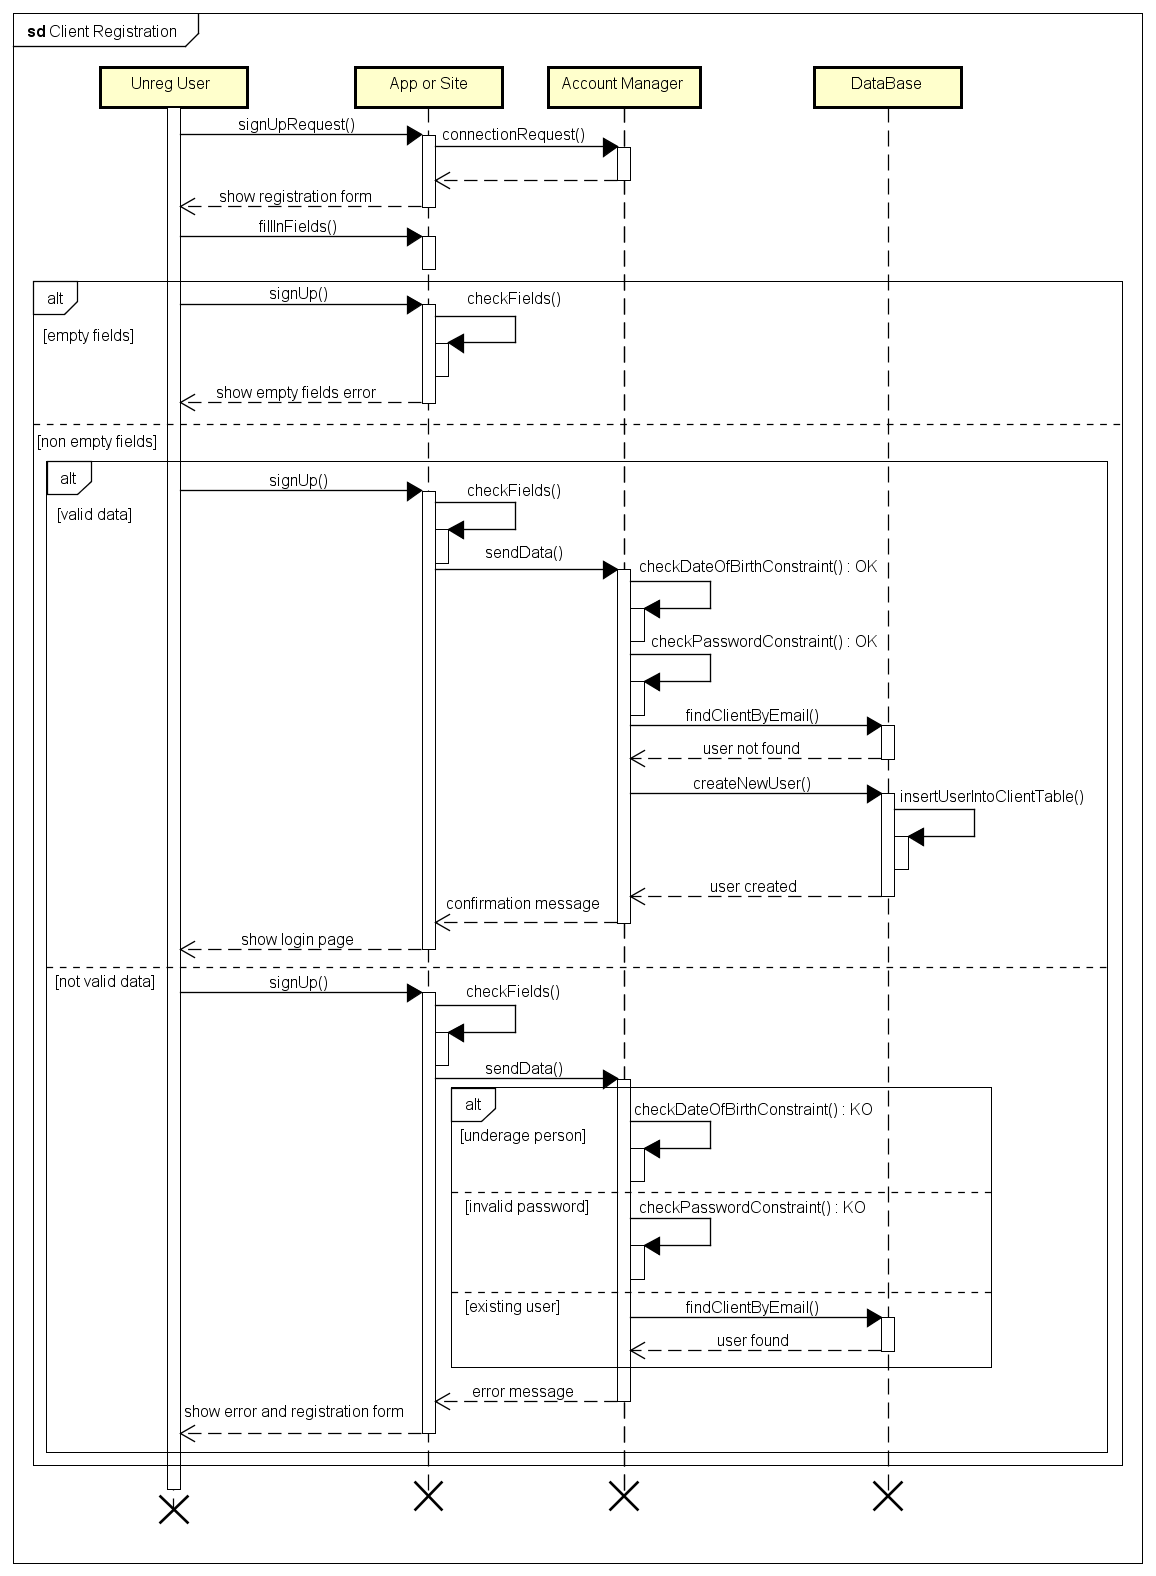
\includegraphics[width=\sequenceWidth]{Sequence-ClientRegistration}
\centering
\caption{Client Registration UML Sequence Diagram}
\label{fig:sequenceclientregistration}
\end{figure}

\begin{figure}[H]
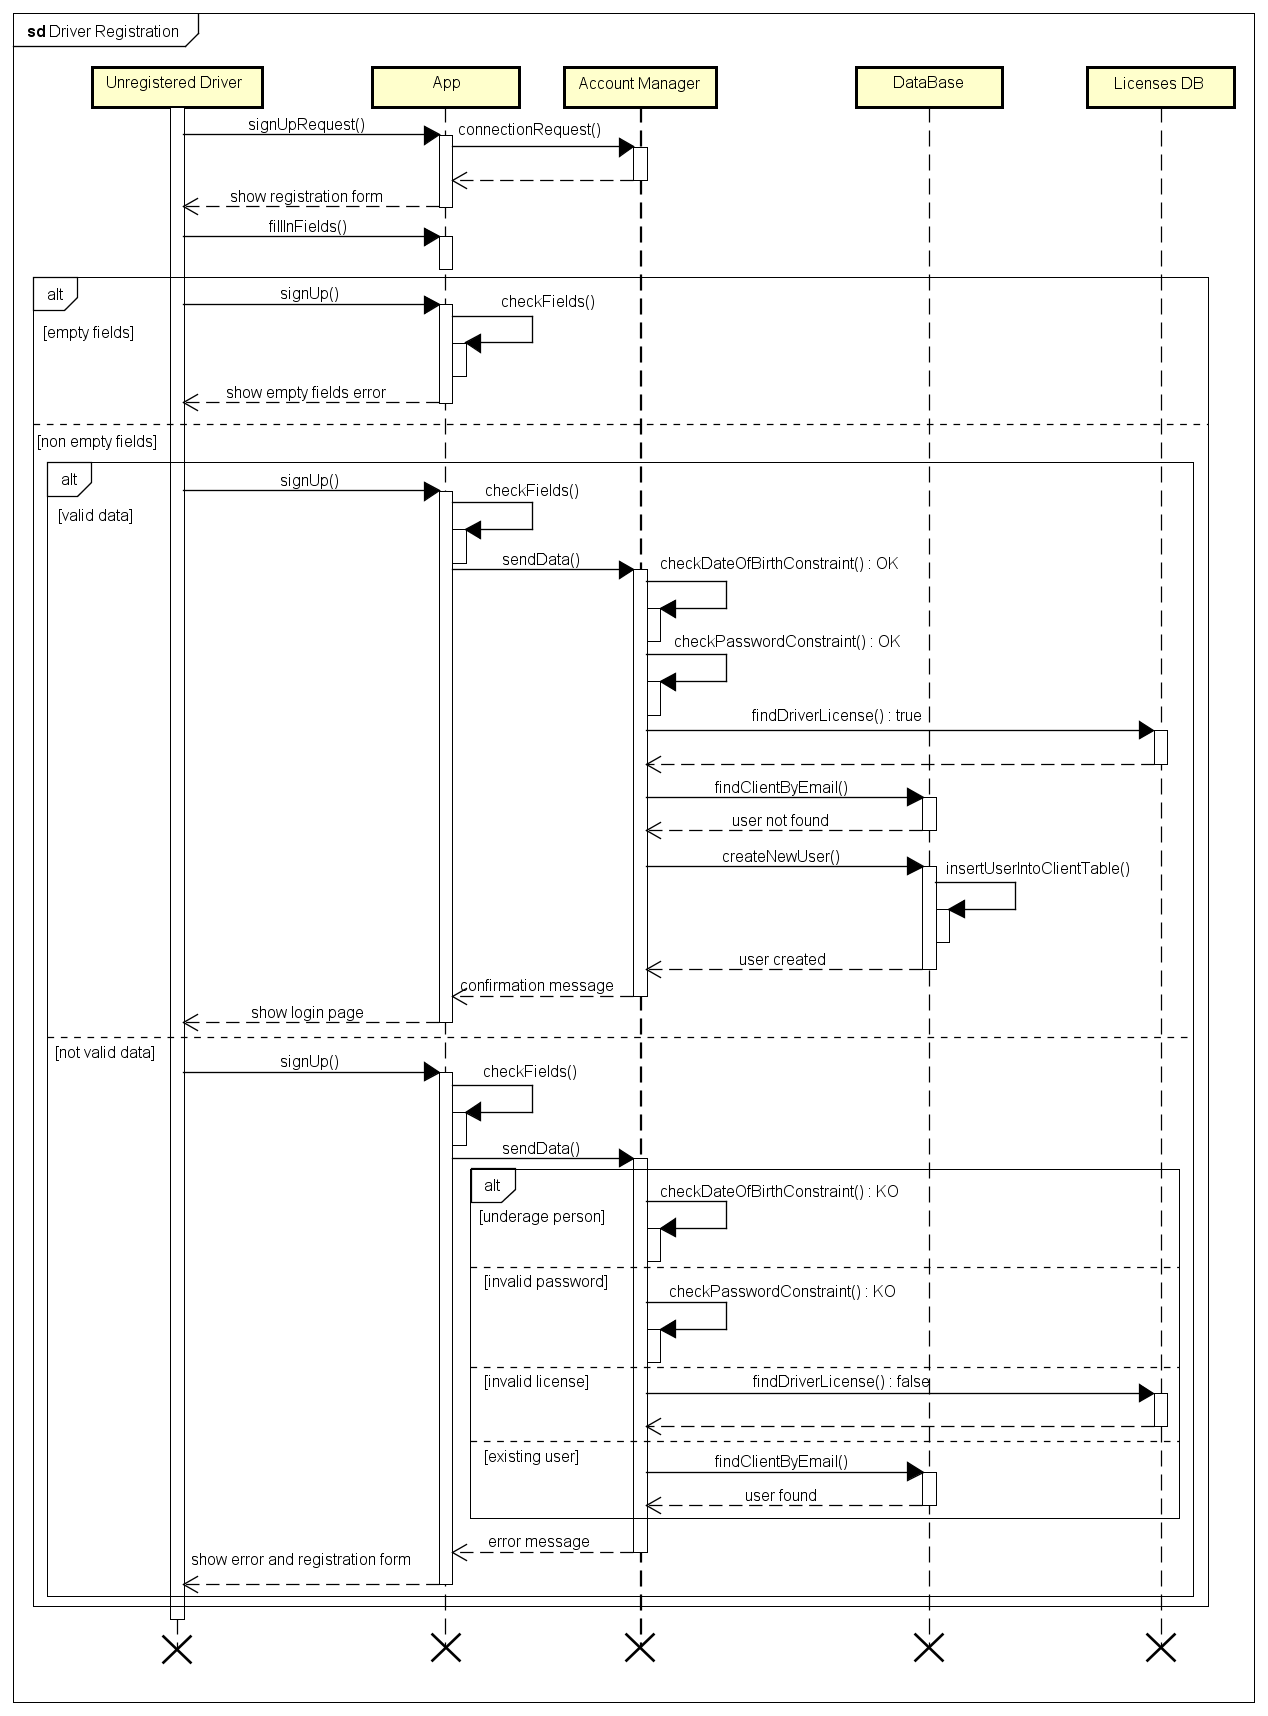
\includegraphics[width=\sequenceWidth]{Sequence-DriverRegistration}
\centering
\caption{Taxi Driver Registration UML Sequence Diagram}
\label{fig:sequencedriverregistration}
\end{figure}

\begin{figure}[H]
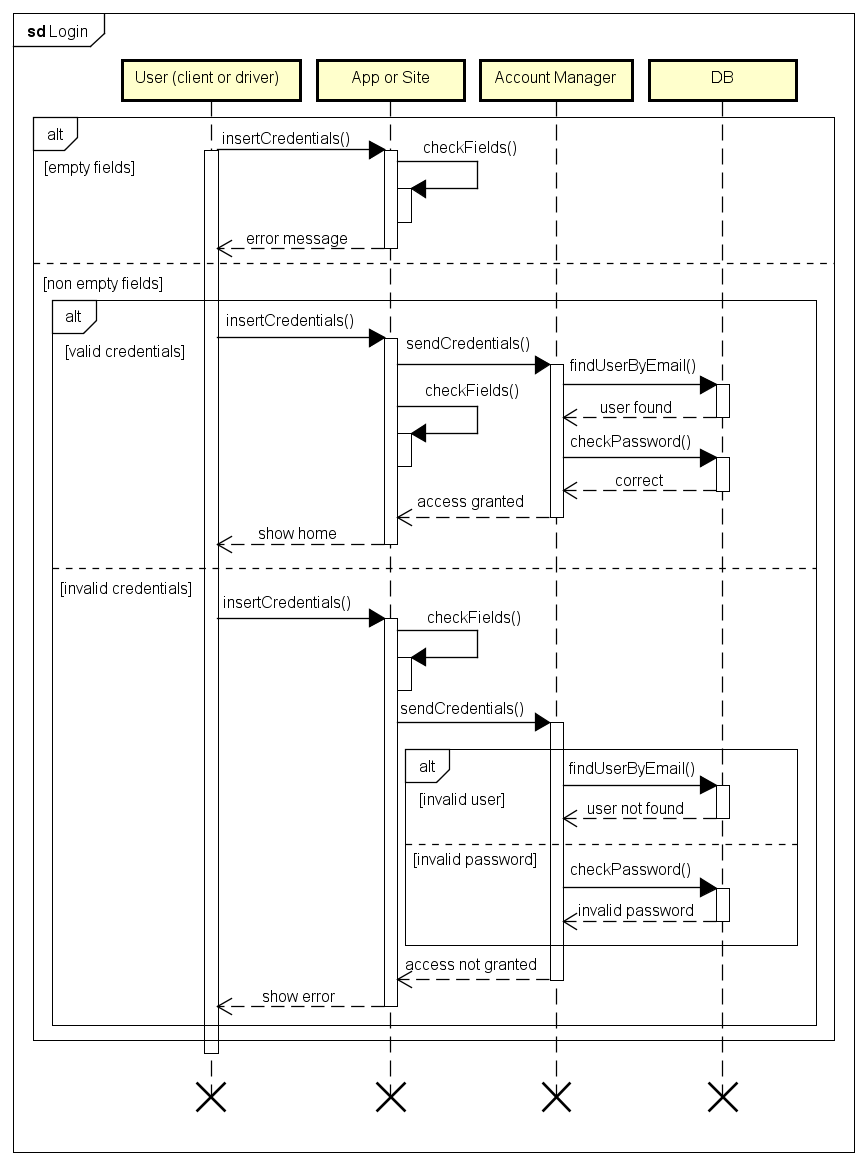
\includegraphics[width=\sequenceWidth]{Sequence-Login}
\centering
\caption{Login UML Sequence Diagram}
\label{fig:sequencelogin}
\end{figure}

\begin{figure}[H]
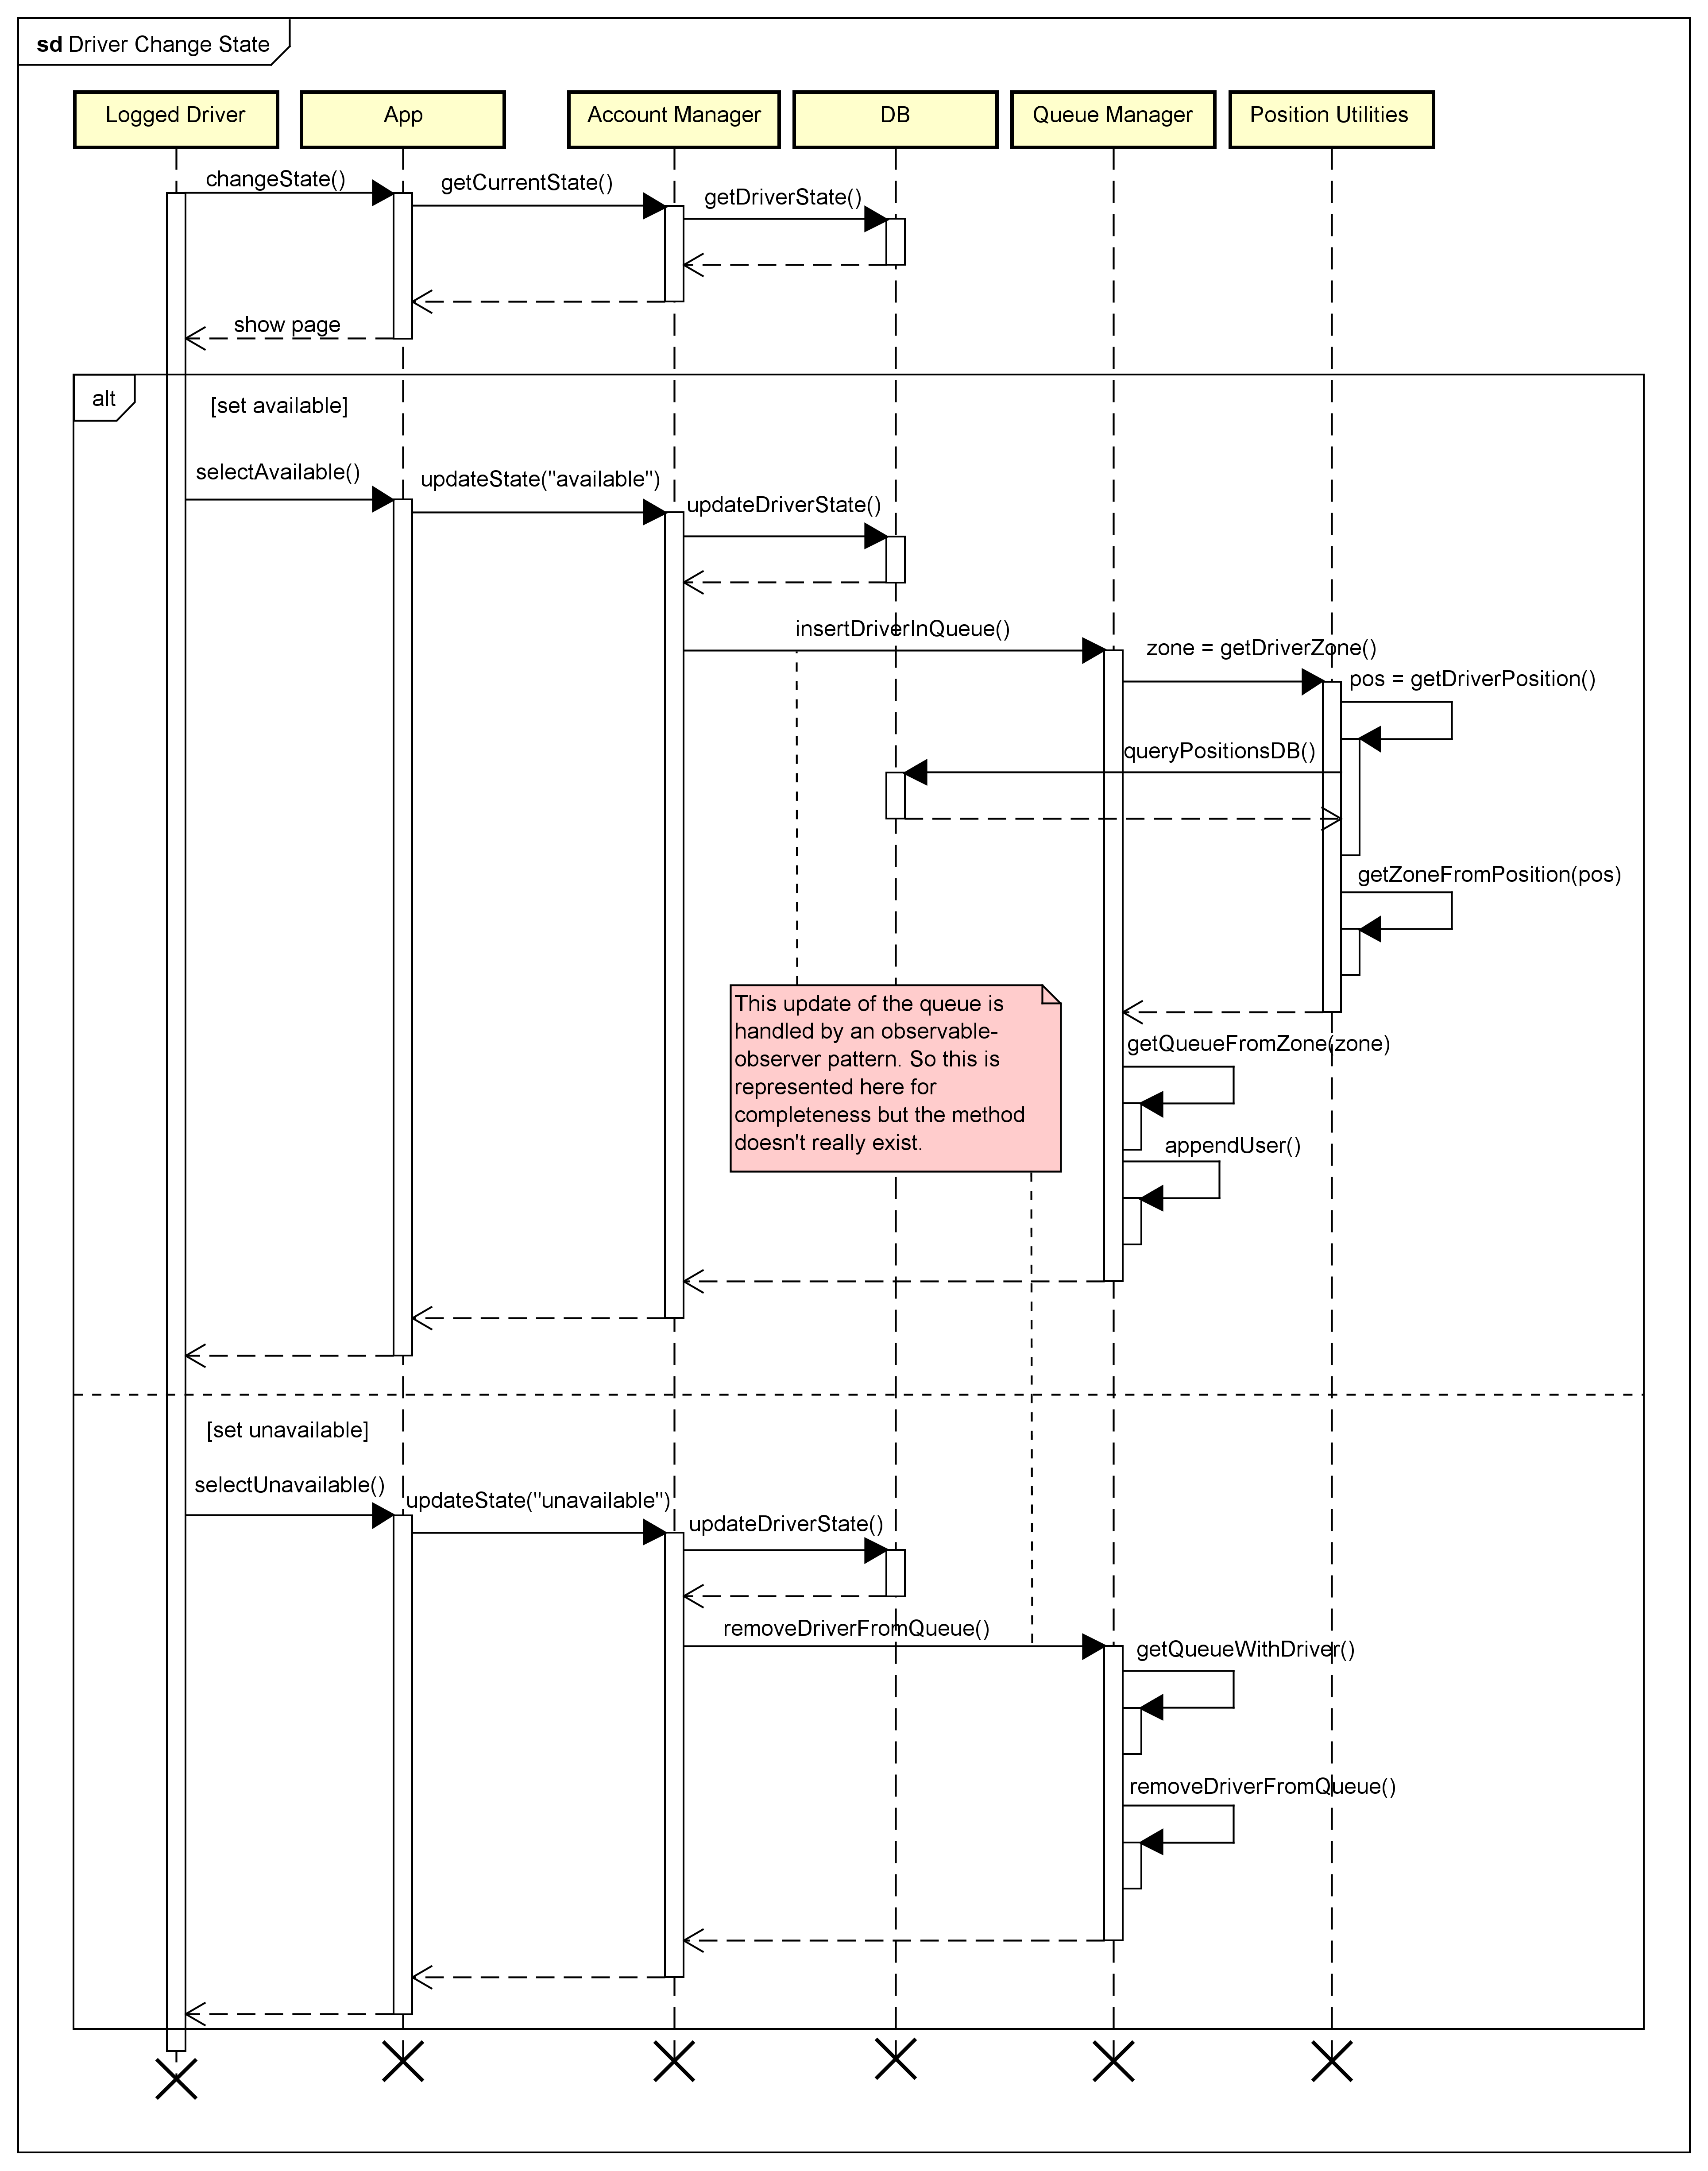
\includegraphics[width=\sequenceWidth]{Sequence-DriverChangeState}
\centering
\caption{Taxi Driver Changes State UML Sequence Diagram}
\label{fig:sequencedriverstate}
\end{figure}

\begin{figure}[H]
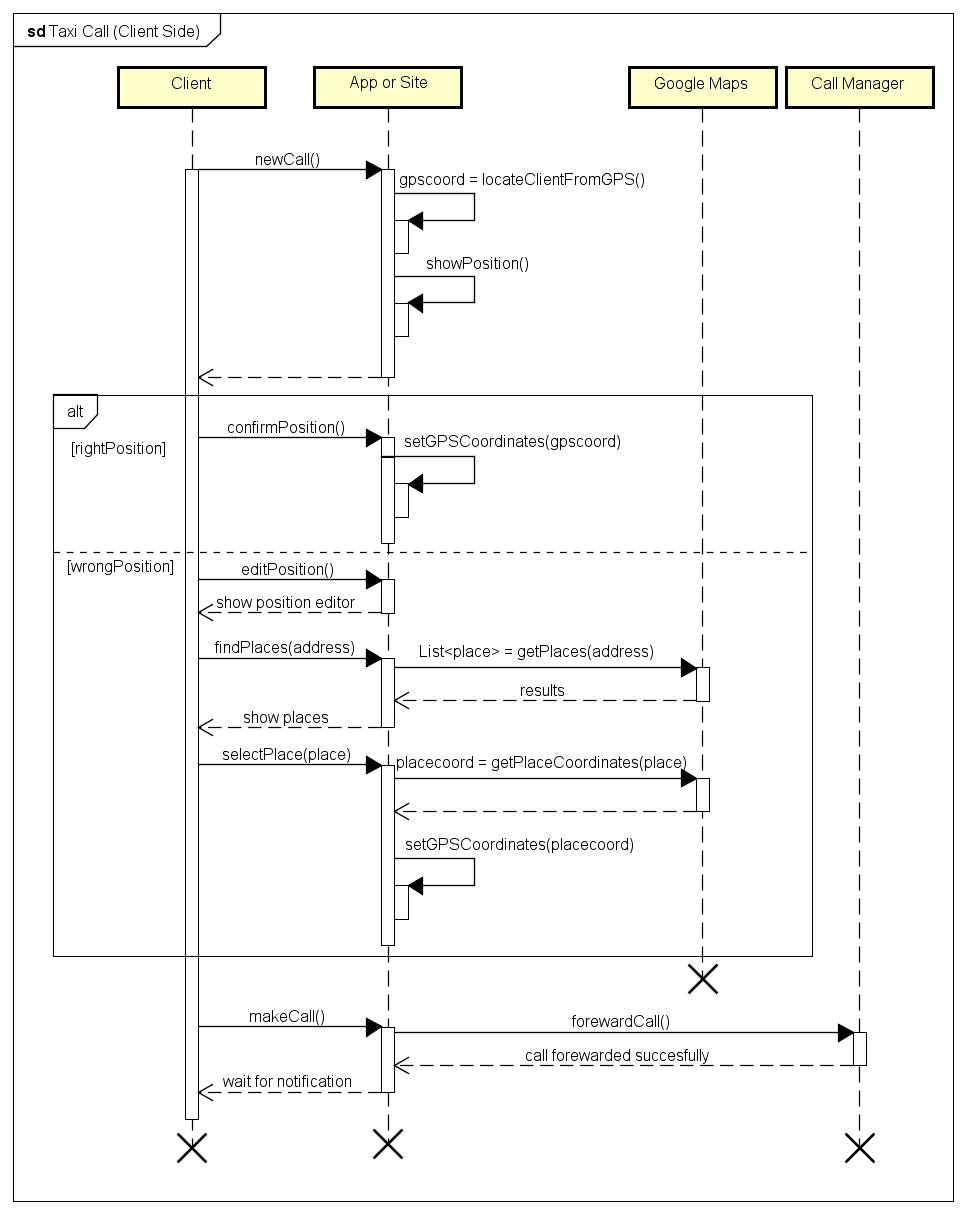
\includegraphics[width=\sequenceWidth]{Sequence-TaxiCallClientSide}
\centering
\caption{Taxi Call Client Side UML Sequence Diagram}
\label{fig:sequencecallclientside}
\end{figure}

\begin{figure}[H]
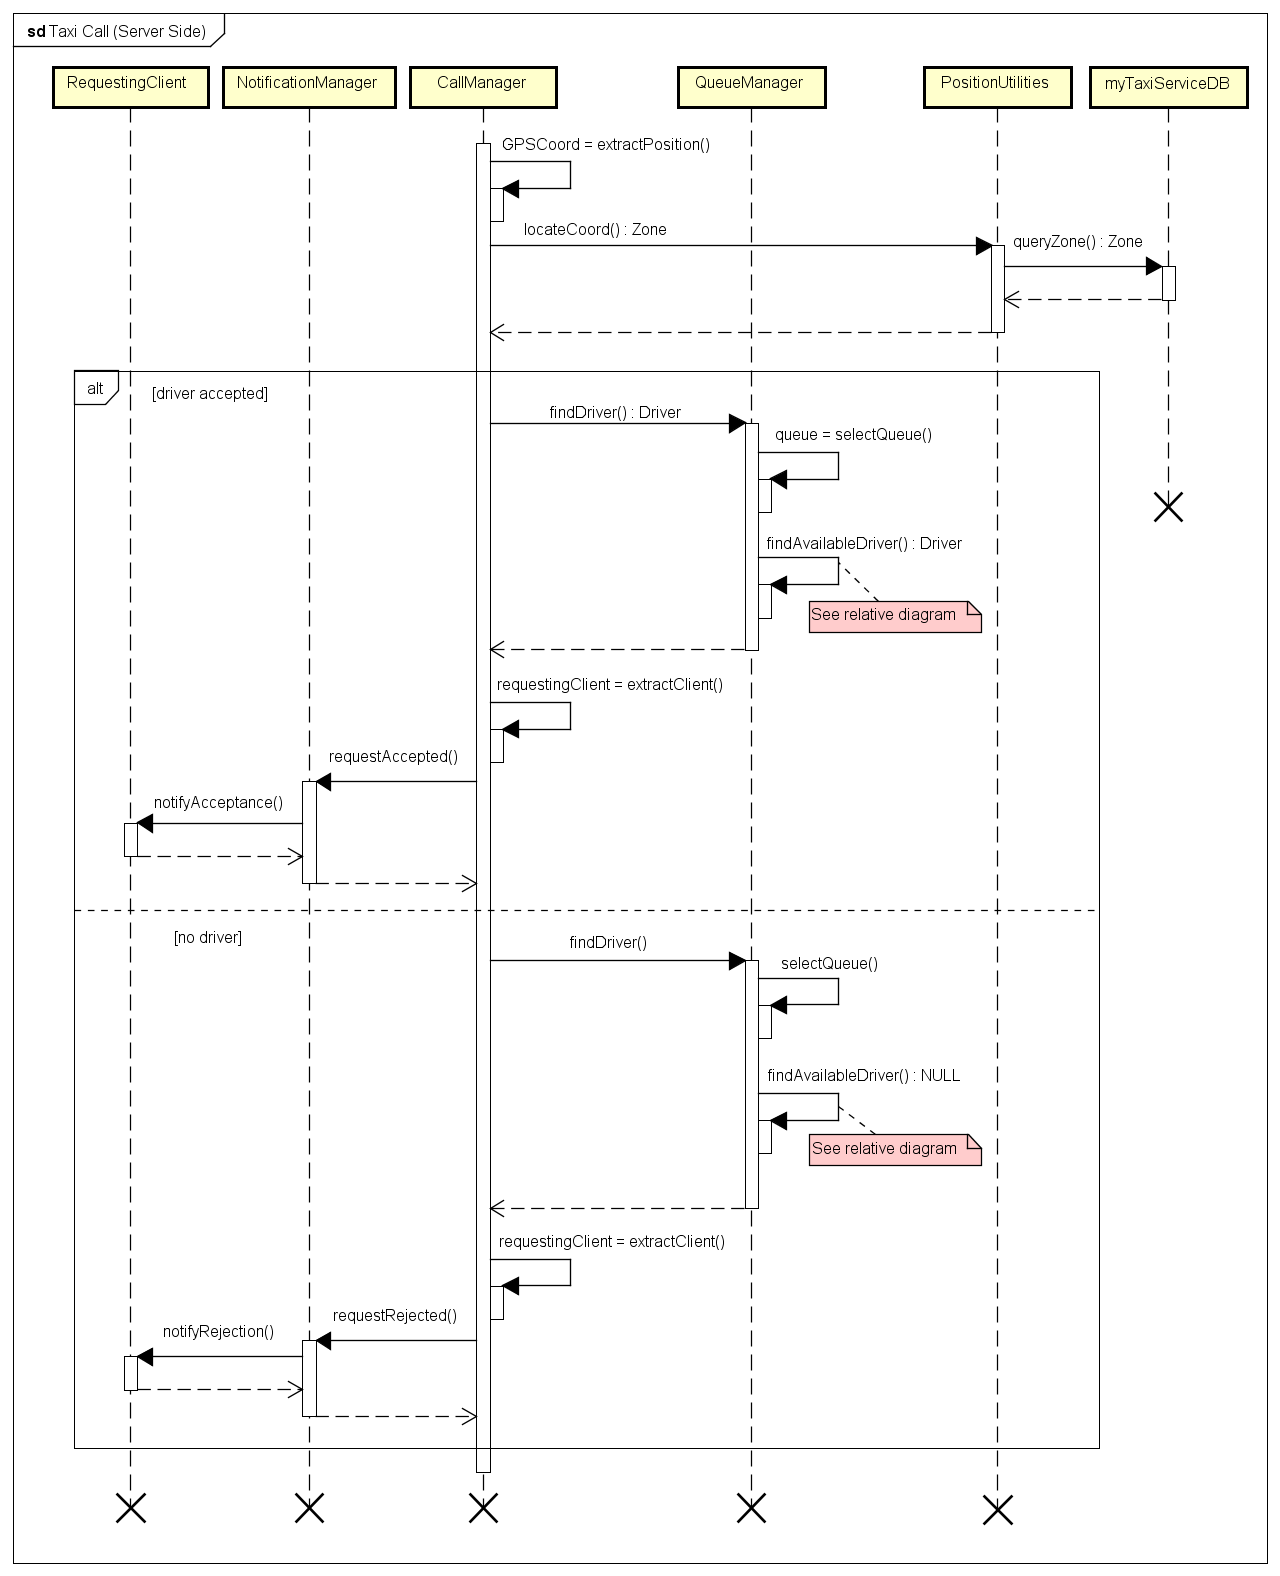
\includegraphics[width=\sequenceWidth]{Sequence-TaxiCallServerSide}
\centering
\caption[Taxi Call Server Side UML Sequence Diagram]{Taxi Call Server Side UML Sequence Diagram: \newline \centering See \autoref{fig:sequencefindavailabledriver} in order to understand what happens in the \emph{findAvailableDriver()} method.}
\label{fig:sequencecallserverside}
\end{figure}

\begin{figure}[H]
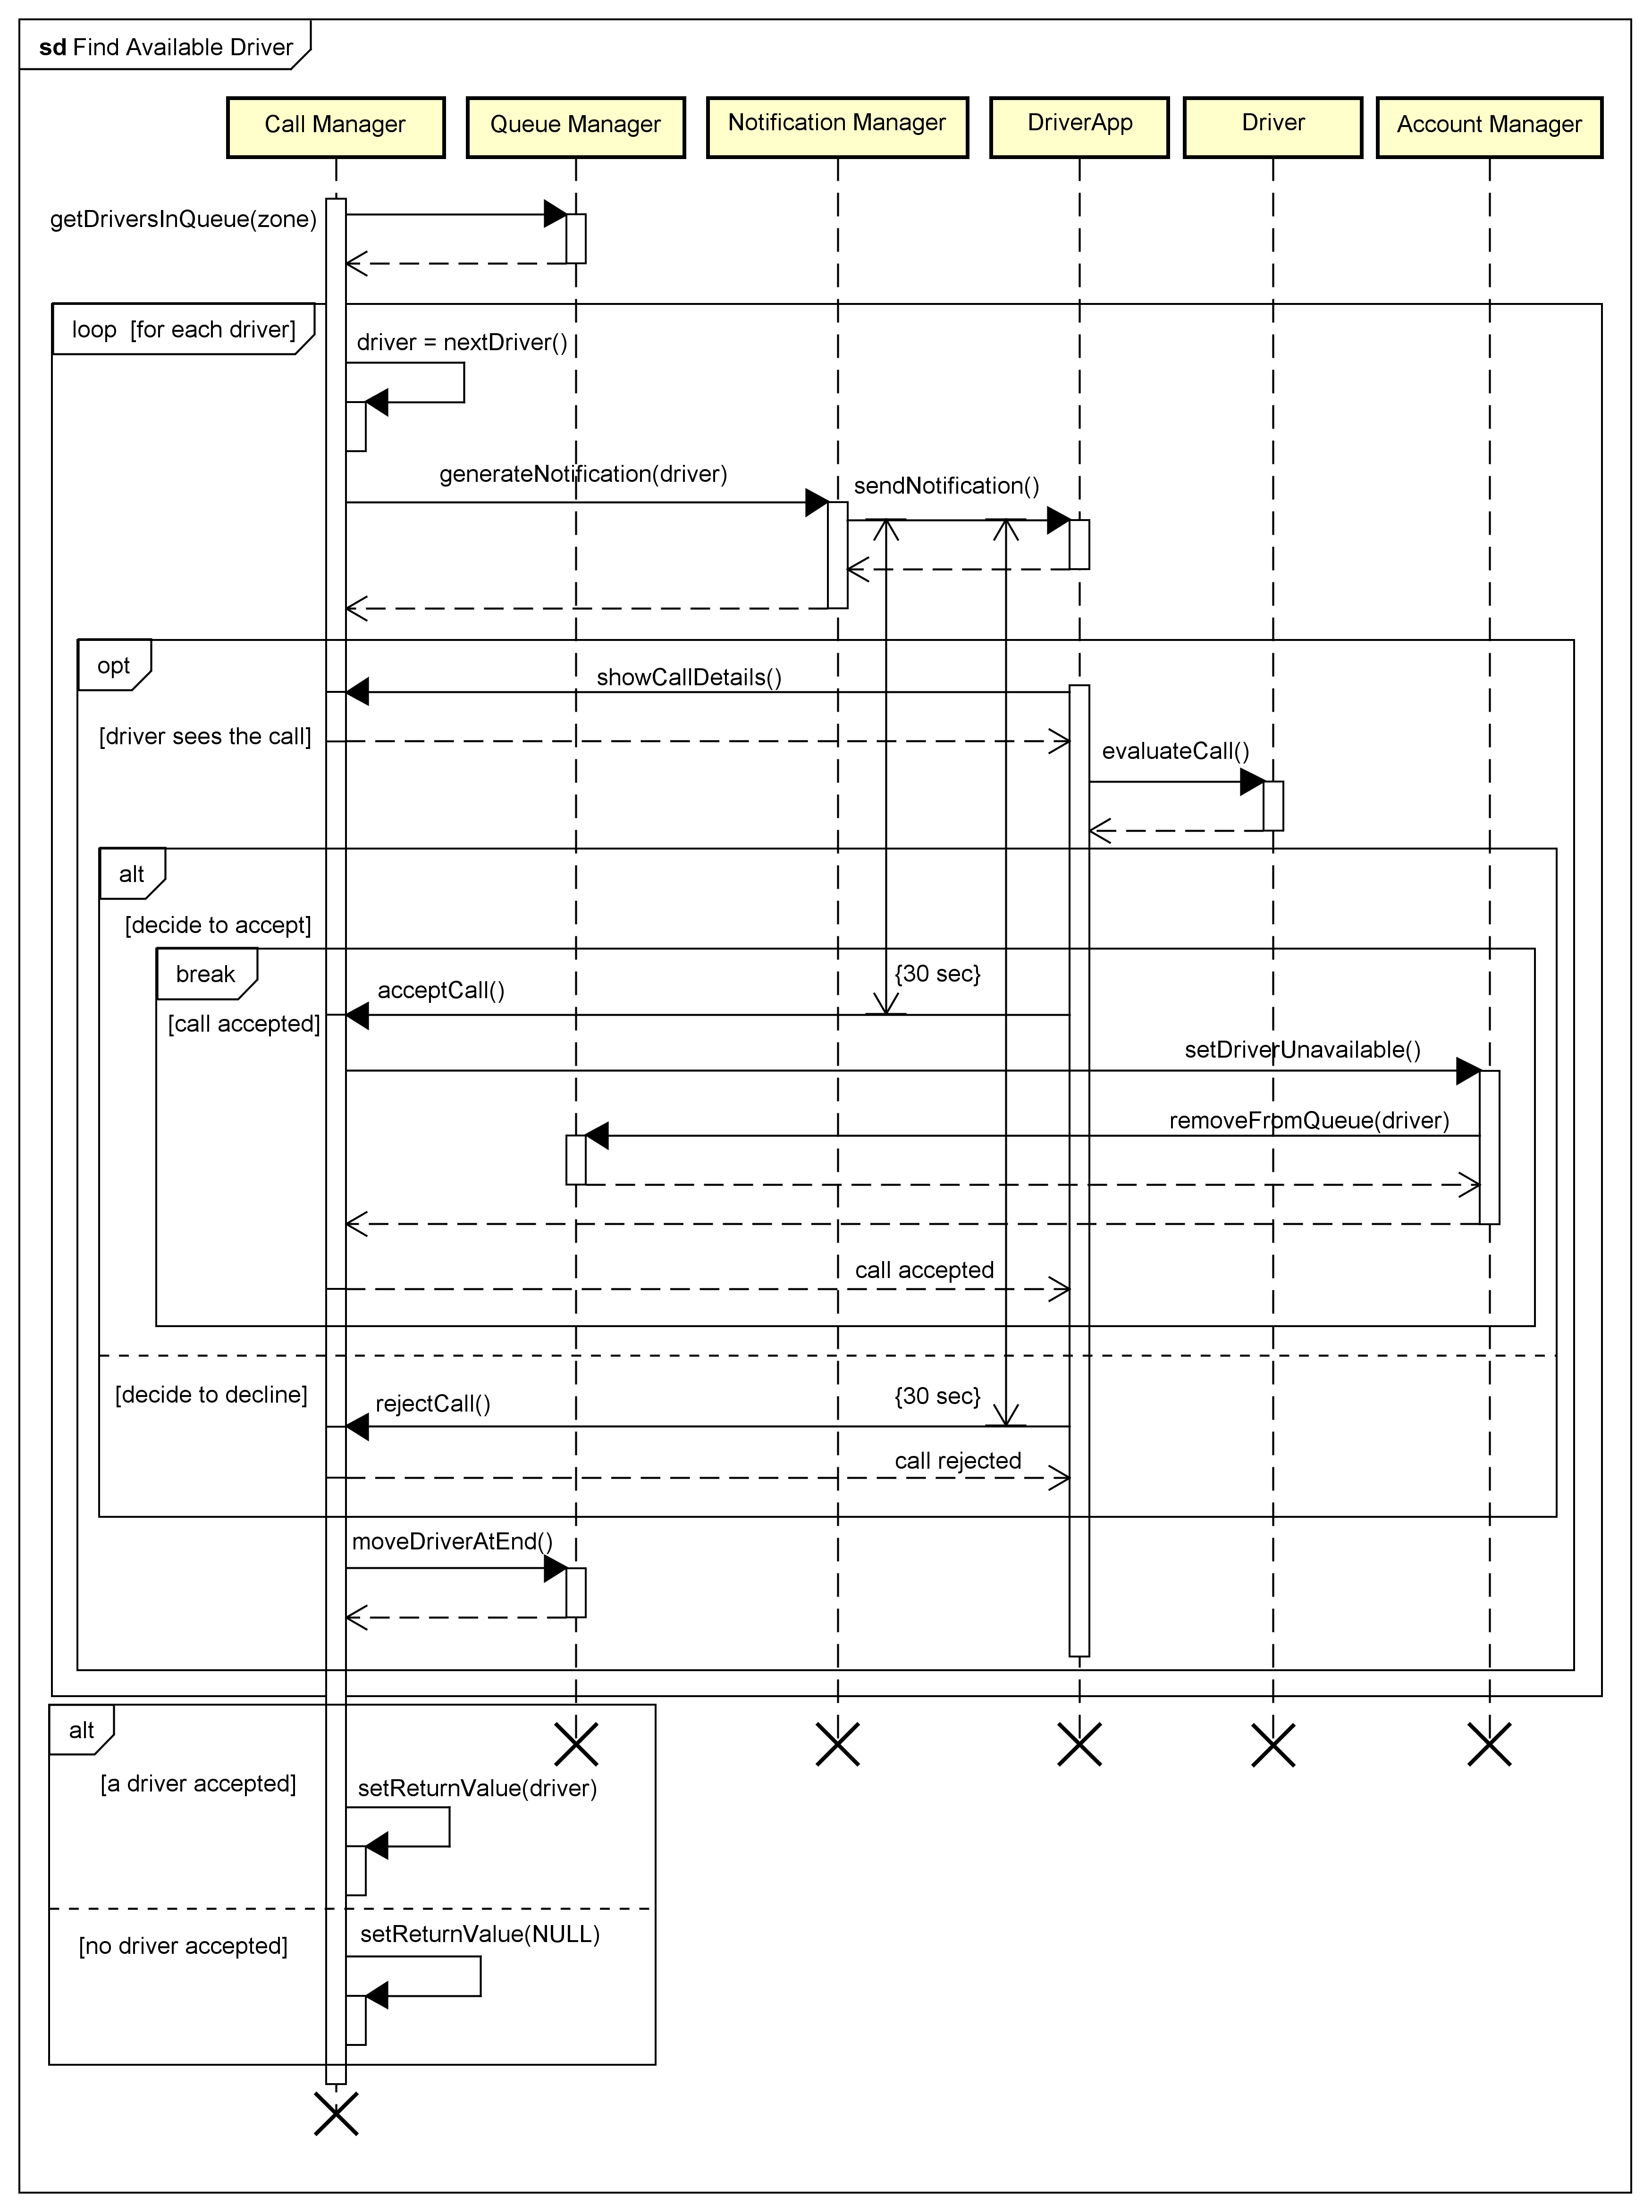
\includegraphics[width=\sequenceWidth]{Sequence-FindAvailableDriver}
\centering
\caption{Find Available Driver UML Sequence Diagram}
\label{fig:sequencefindavailabledriver}
\end{figure}

\begin{figure}[H]
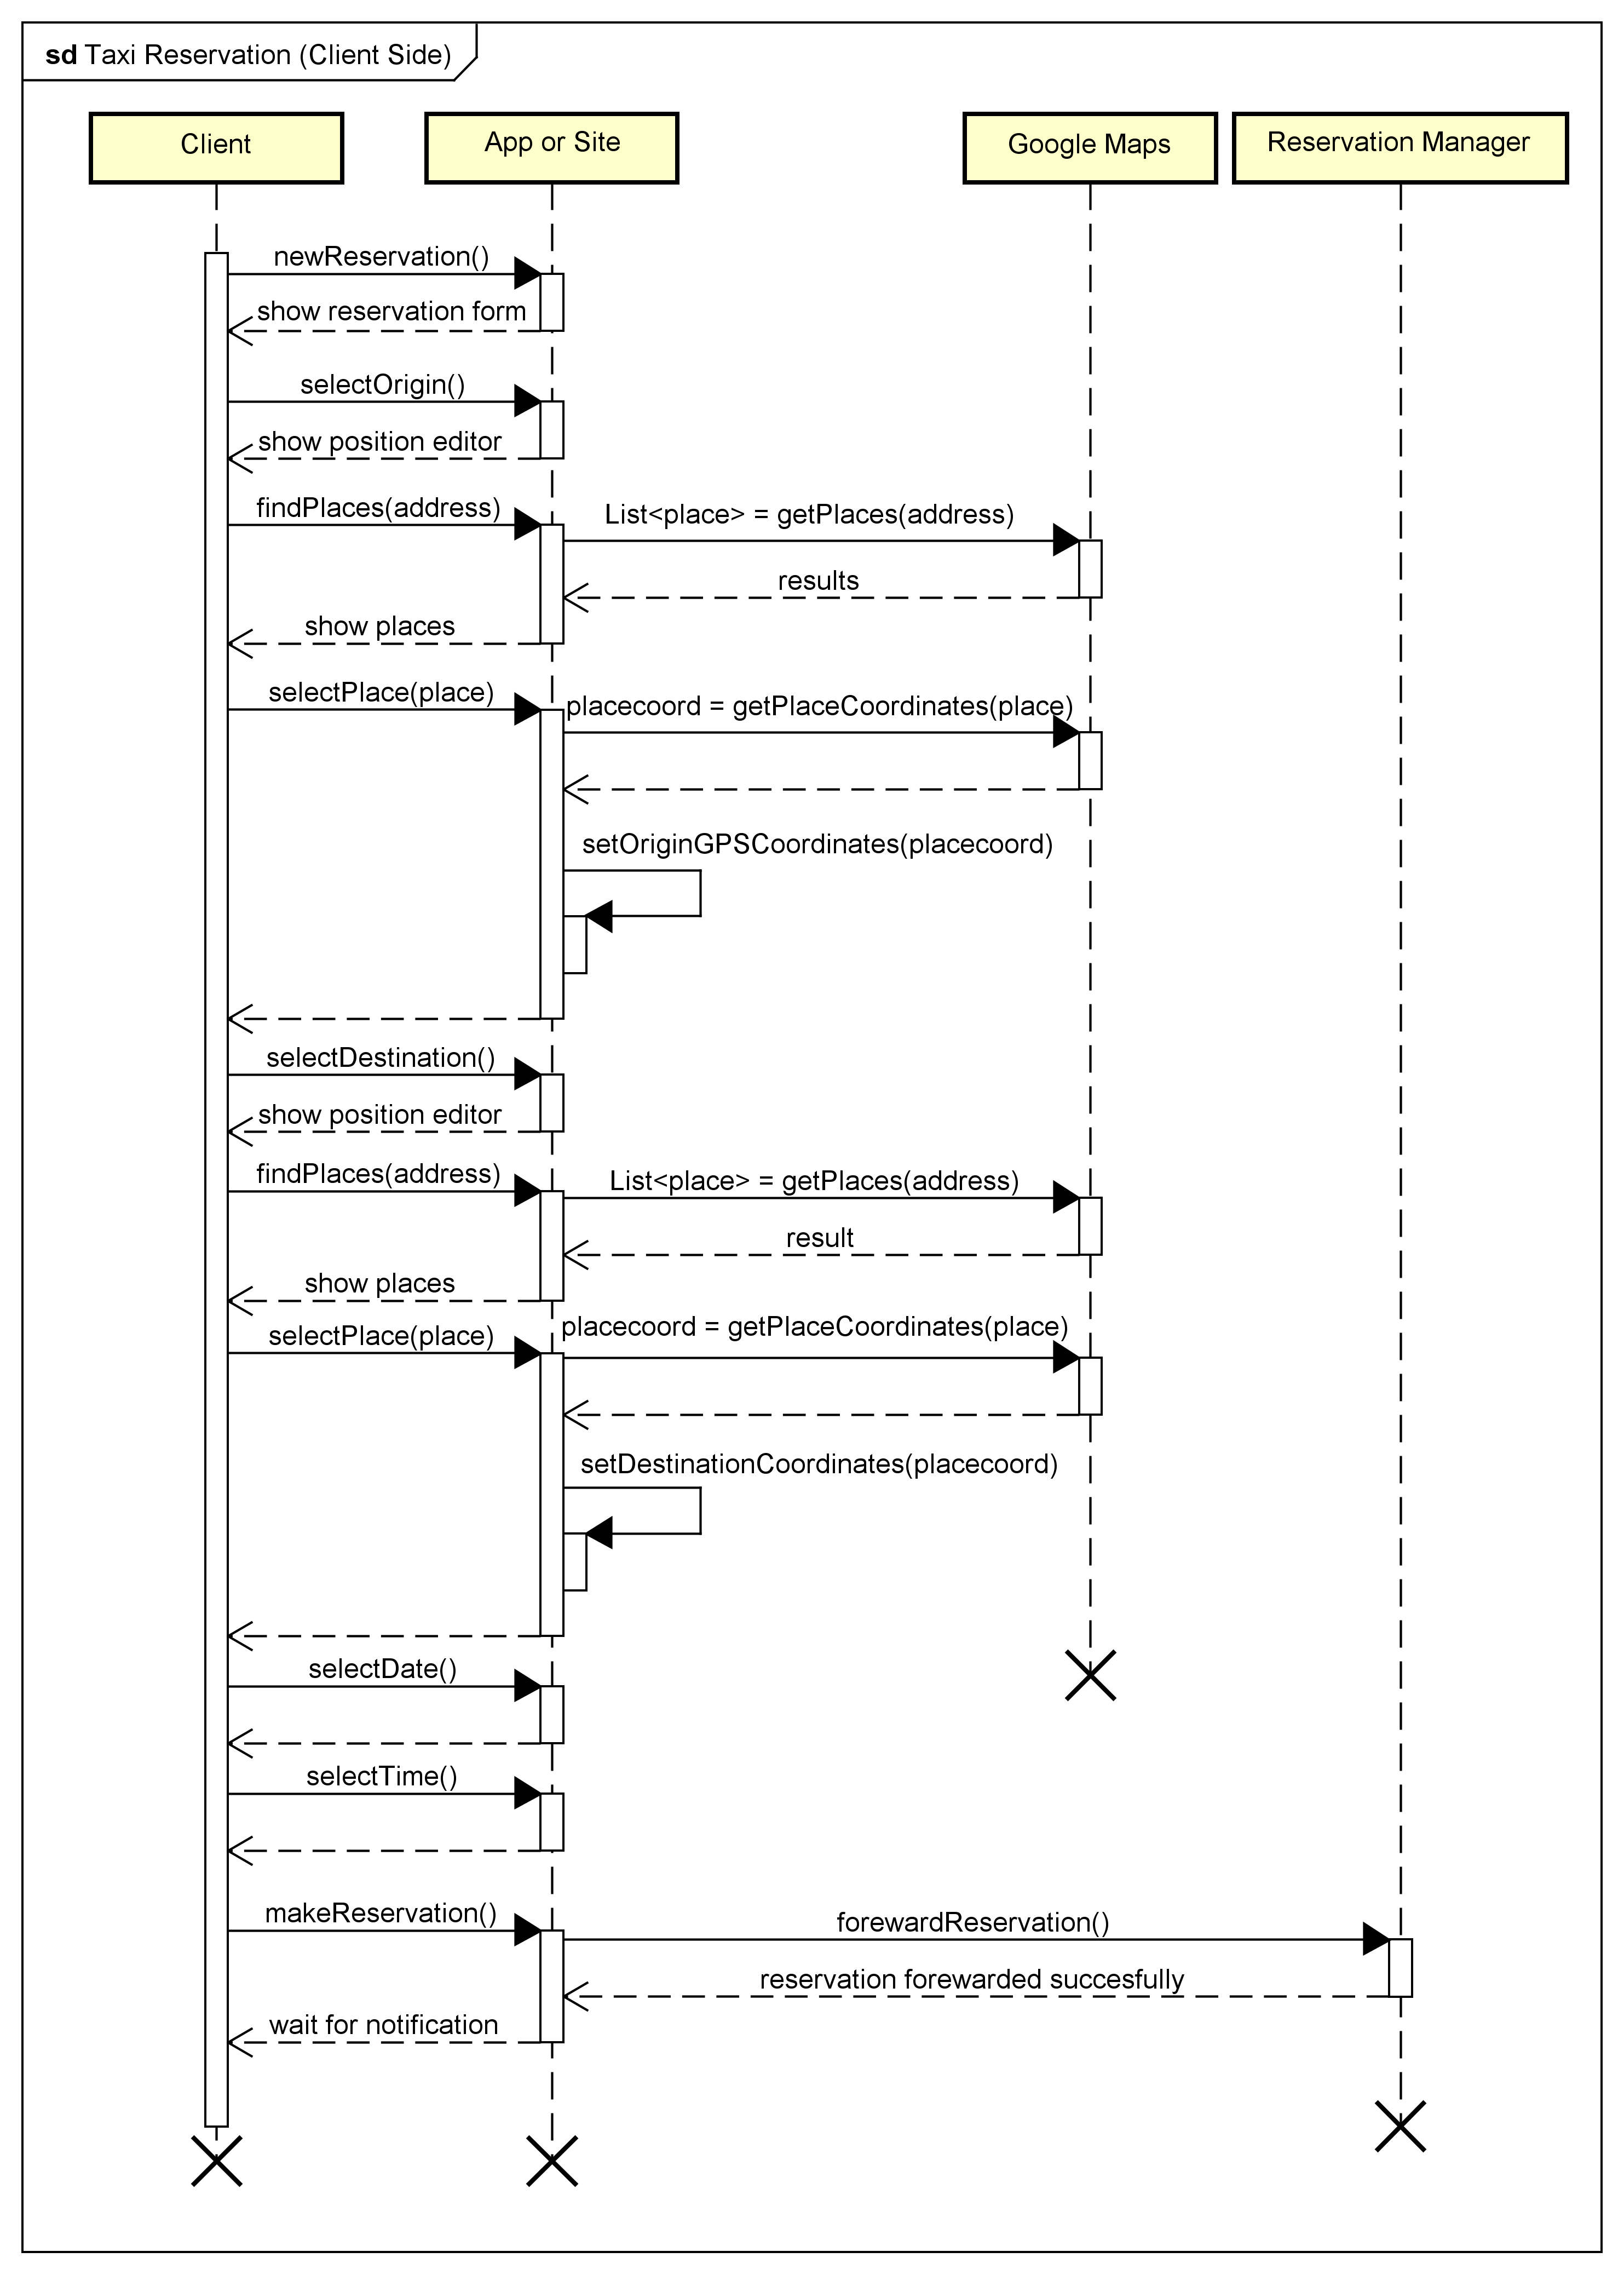
\includegraphics[width=\sequenceWidth]{Sequence-TaxiReservationClientSide}
\centering
\caption{Taxi Reservation Client Side UML Sequence Diagram}
\label{fig:sequencereservationclientside}
\end{figure}

\begin{figure}[H]
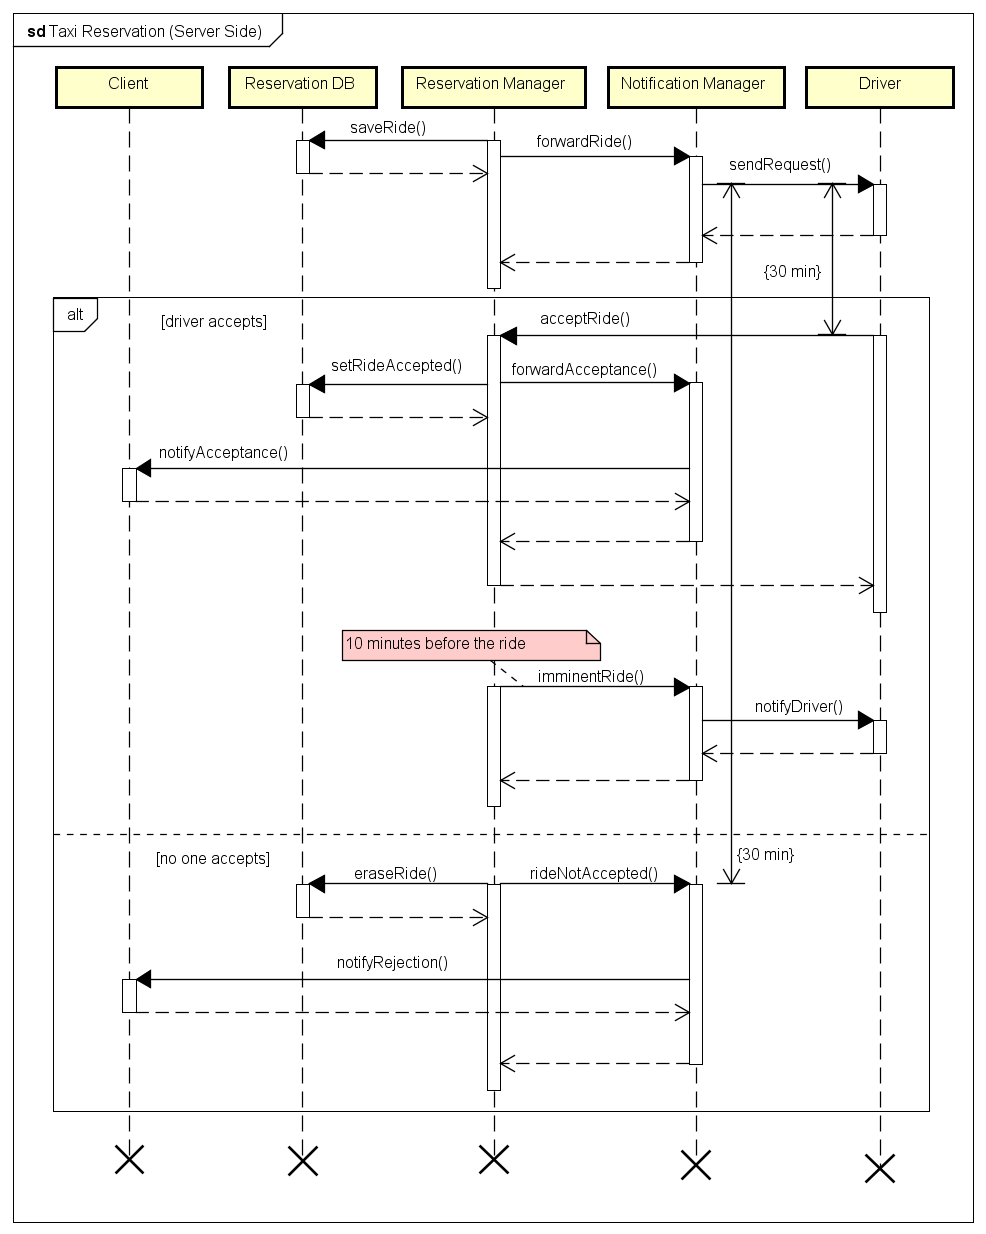
\includegraphics[width=\sequenceWidth]{Sequence-TaxiReservationServerSide}
\centering
\caption{Taxi Reservation Server Side UML Sequence Diagram}
\label{fig:sequencereservationserverside}
\end{figure}

\begin{figure}[H]
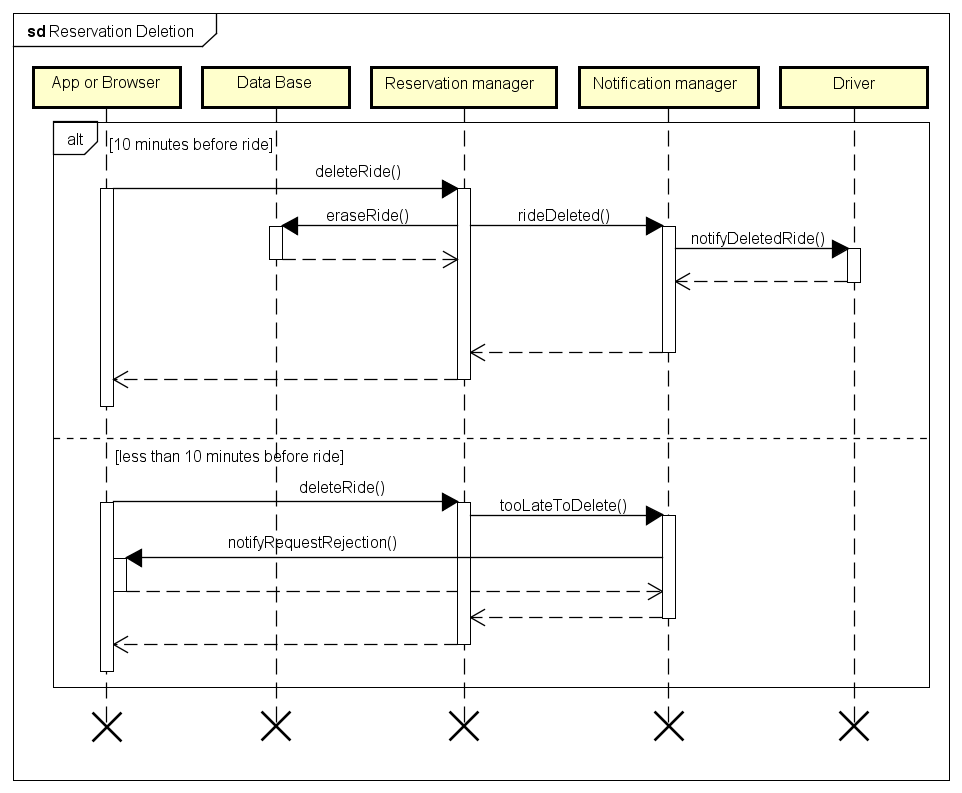
\includegraphics[width=\sequenceWidth]{Sequence-TaxiReservationDeletion}
\centering
\caption{Taxi Reservation Deletion UML Sequence Diagram}
\label{fig:sequencereservationdeletion}
\end{figure}

\subsection{Component Interfaces}
\subsection{Selected Architectural Styles and Patterns}

\section{Requirements traceability}
\begin{table} [H]
\begin{center}
\begin{tabular}{ |m{.25\textwidth}|m{.65\textwidth}|  }
\hline
    \multicolumn{2}{|c|}{\textbf{\textit{The client receives a Taxi Call Confirmation}}} \\
\hline \hline
    \textbf{Actors}
&   Registered Client
\\ \hline
    \textbf{Entry Conditions}
&   The Client must be logged into the website or the application.
\\ \hline
    \textbf{Flow of Events}
& 
    \begin{enumerate*}
    \item The client receives a notification
    \item The app (or website) shows the number of the taxi which will arrive, the taxi driver's phone number and the waiting time
    \end{enumerate*}
\\ \hline
    \textbf{Exit Conditions}
&   The call will arrive in the specified waiting time.
\\ \hline
    \textbf{Exceptions}
&   
    There are not exceptions for this use case.
\\ \hline
\end{tabular}
\end{center}
\caption{Use Case Description of a Taxi Call Confirmation}
\label{table:clientconfirmation}
\end{table}
\end{document}
